\documentclass[tikz,border=5pt]{standalone}
\usepackage{tikz}
\usetikzlibrary{shapes,arrows,positioning,calc}

\begin{document}
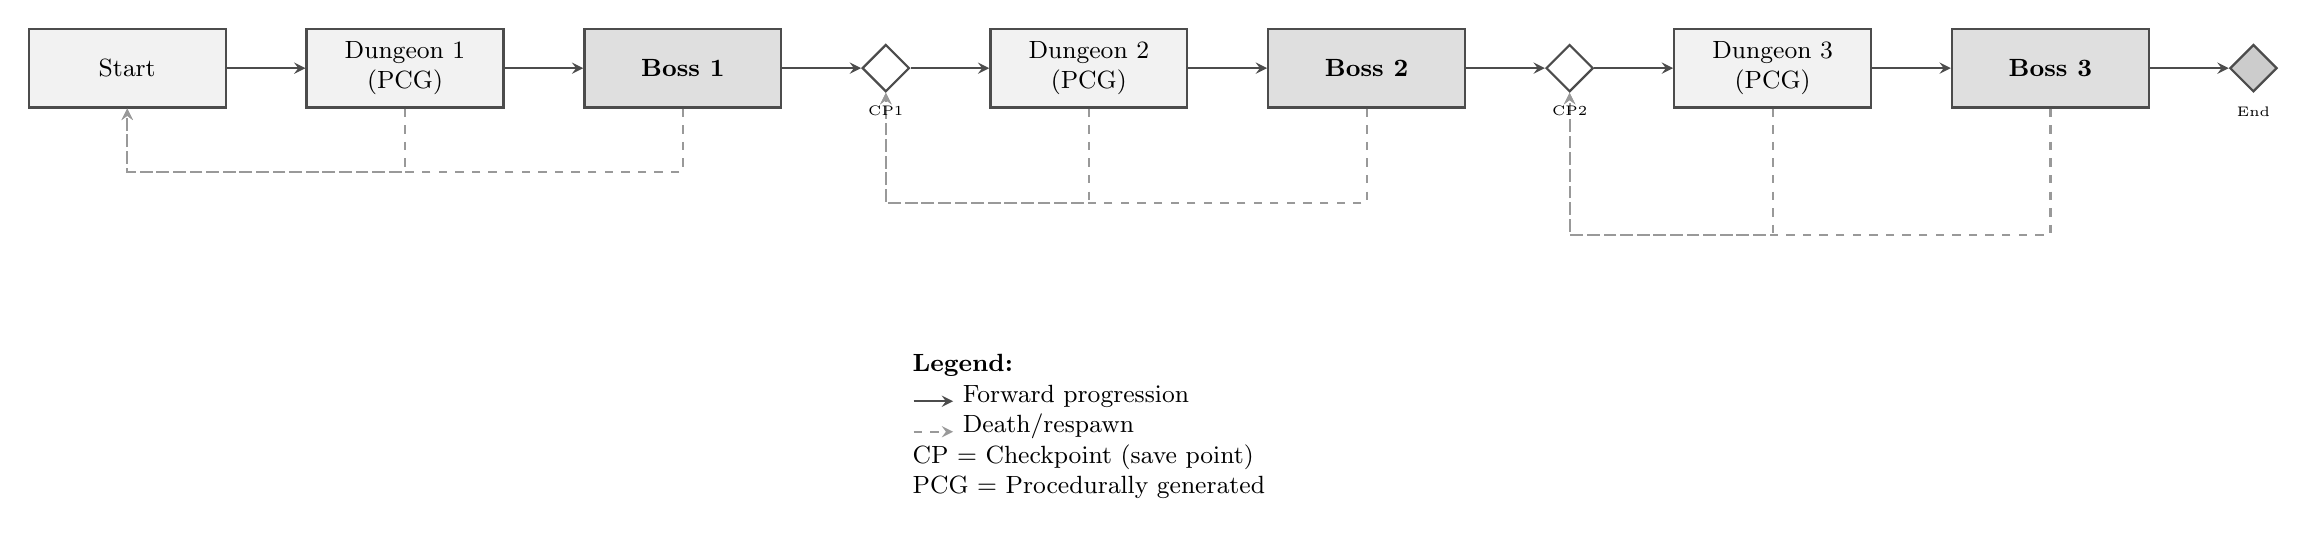
\begin{tikzpicture}[
    node distance=1.5cm and 1cm,
    dungeon/.style={rectangle, draw=black!70, fill=gray!10, thick, minimum width=2.5cm, minimum height=1cm, align=center, font=\small},
    boss/.style={rectangle, draw=black!70, fill=gray!25, thick, minimum width=2.5cm, minimum height=1cm, align=center, font=\small\bfseries},
    checkpoint/.style={diamond, draw=black!70, fill=white, thick, minimum size=0.6cm, inner sep=0pt},
    arrow/.style={->, >=stealth, thick, black!70},
    death/.style={->, >=stealth, thick, black!40, dashed}
    ]

    % Row 1: Main progression path
    \node[dungeon] (start) {Start};
    \node[dungeon, right=of start] (d1) {Dungeon 1\\(PCG)};
    \node[boss, right=of d1] (b1) {Boss 1};
    \node[checkpoint, right=of b1] (c1) {};

    \node[dungeon, right=of c1] (d2) {Dungeon 2\\(PCG)};
    \node[boss, right=of d2] (b2) {Boss 2};
    \node[checkpoint, right=of b2] (c2) {};

    \node[dungeon, right=of c2] (d3) {Dungeon 3\\(PCG)};
    \node[boss, right=of d3] (b3) {Boss 3};
    \node[checkpoint, right=of b3, fill=gray!40] (victory) {};

    % Forward progression arrows
    \draw[arrow] (start) -- (d1);
    \draw[arrow] (d1) -- (b1);
    \draw[arrow] (b1) -- (c1);
    \draw[arrow] (c1) -- (d2);
    \draw[arrow] (d2) -- (b2);
    \draw[arrow] (b2) -- (c2);
    \draw[arrow] (c2) -- (d3);
    \draw[arrow] (d3) -- (b3);
    \draw[arrow] (b3) -- (victory);

    % Death respawn paths
    \draw[death] (d1.south) -- ++(0,-0.8) -| (start.south);
    \draw[death] (b1.south) -- ++(0,-0.8) -| (start.south);

    \draw[death] (d2.south) -- ++(0,-1.2) -| (c1.south);
    \draw[death] (b2.south) -- ++(0,-1.2) -| (c1.south);

    \draw[death] (d3.south) -- ++(0,-1.6) -| (c2.south);
    \draw[death] (b3.south) -- ++(0,-1.6) -| (c2.south);

    % Labels
    \node[below=0.05cm of c1, font=\tiny] {CP1};
    \node[below=0.05cm of c2, font=\tiny] {CP2};
    \node[below=0.05cm of victory, font=\tiny] {End};

    % Legend
    \node[below=3cm of d2, font=\small, align=left] {
        \textbf{Legend:}\\
        \tikz{\draw[arrow] (0,0) -- (0.5,0);} Forward progression\\
        \tikz{\draw[death] (0,0) -- (0.5,0);} Death/respawn\\
        CP = Checkpoint (save point)\\
        PCG = Procedurally generated
    };

\end{tikzpicture}
\end{document}
